\chapter{Deskriptive Analyse \textit{\textcolor{gray}{(Autoren: Philipp und Patrick)}}}

%Betrachtung was in den Daten enthalten ist (Geschlechter Verteilung, Alter, etc.)
In der durchgeführten wurden zu Beginn allgemeine Daten über die Teilnehmenden erhoben.
Die Informationen welche über die Teilnehmenden abgefragt worden sind, können in der Tabelle
\ref{tab:allgemeine_daten} eingesehen werden.

% \usepackage{float}
\begin{table}[h]
    \centering
    \begin{tabular}{|l|l|p{8cm}|}
        \hline
        \textbf{Variable} & \textbf{Frage} & \textbf{Bedeutung}\\
        \hline
        Geschlecht & QA1 & Welchem Geschlecht fühlt sich die Person angehörig\\\hline
        Alter & QA2 & In Gruppen von 10 Jahren (Bsw. 16-25, 26-35, 66+)\\\hline
        Kinder & QA3 & Hat die Person Kinder\\\hline
        Vollzeit/Teilzeit & QA7 & Ist die Person in Vollzeit oder Teilzeit tätig\\\hline
        Körperliche Beanspruchung & QA11 & Wie stark ist die körperliche Belastung der Arbeit\\\hline
        Branche & QA12 & In welcher Branche ist die Person tätig\\\hline
        Bereits 4TW & QA16 & Hat die Person bereits eine 4-Tage-Woche\\\hline
    \end{tabular}
    \caption{Allgemeine Daten der Teilnehmenden}
    \label{tab:allgemeine_daten}
\end{table}

Mit den Informationen kann zum einen eine allgemeine Aussage über die Gruppe der Teilnehmenden 
getroffen werden, als auch zu den Hypothesen im den Kapiteln \ref{chap:hypothese4},
\ref{chap:hypothese5} und \ref{chap:hypothese9}. Dadurch kann in diesem Kapitel auch betrachtet
werden, ob die Stichprobe repräsentativ ist und ob es besondere Ausprägungen in den Daten gibt.

\begin{figure}[h]
    \centering
    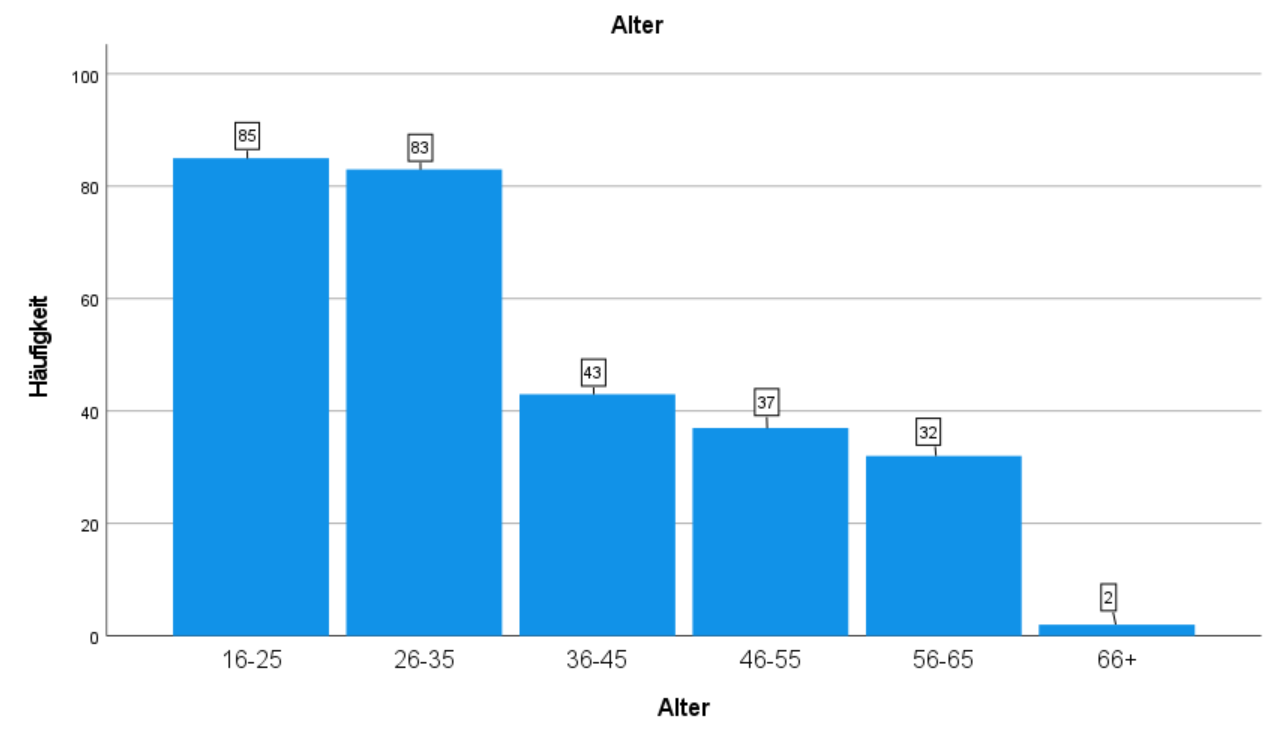
\includegraphics[width=0.7\textwidth]{04_Artefakte/01_Abbildungen/deskriptiv_alter.png}
    \caption{Altersverteilung der Teilnehmenden}
    \label{fig:altersverteilung}
\end{figure}

\begin{figure}[h]
    \centering
    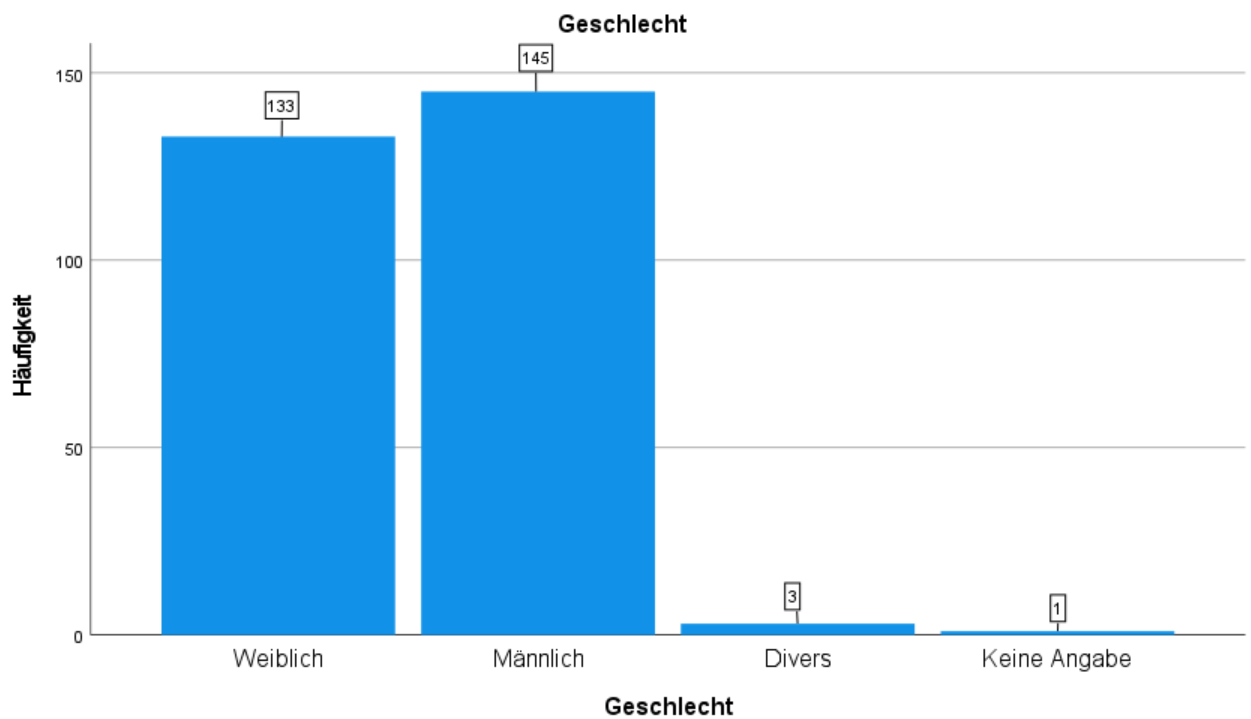
\includegraphics[width=0.8\textwidth]{04_Artefakte/01_Abbildungen/deskriptiv_geschlecht.png}
    \caption{Geschlechterverteilung der Teilnehmenden}
    \label{fig:geschlechterverteilung}
\end{figure}

Zu diesem Zweck wird mit der Betrachtung der Altersverteilung und des Geschlechts der Teilnehmenden sowie des Anteils der Eltern begonnen.
Wie in Abbildung \ref{fig:altersverteilung} zu sehen ist, besteht die Gruppe der Teilnehmenden hauptsächlich aus Personen im Alter von 16 bis 35 Jahren.
Dabei ist die Gruppe der 16 bis 25 Jährigen leicht stärker vertreten als die Gruppe der 26 bis 35 Jährigen.

Bei den Geschlechtern sieht die Verteilung wie in Abbildung \ref{fig:geschlechterverteilung} dargestellt aus. Es gab mit 145 männlichen und 133 weiblichen Personen leicht
mehr Männer als Frauen in der Umfrage. Dazu kamen noch 3 Personen, die sich als divers identifiziert haben und 1 Person, die keine Angabe gemacht hat.

\begin{figure}[h]
    \begin{subfigure}{0.49\textwidth}
        \centering
        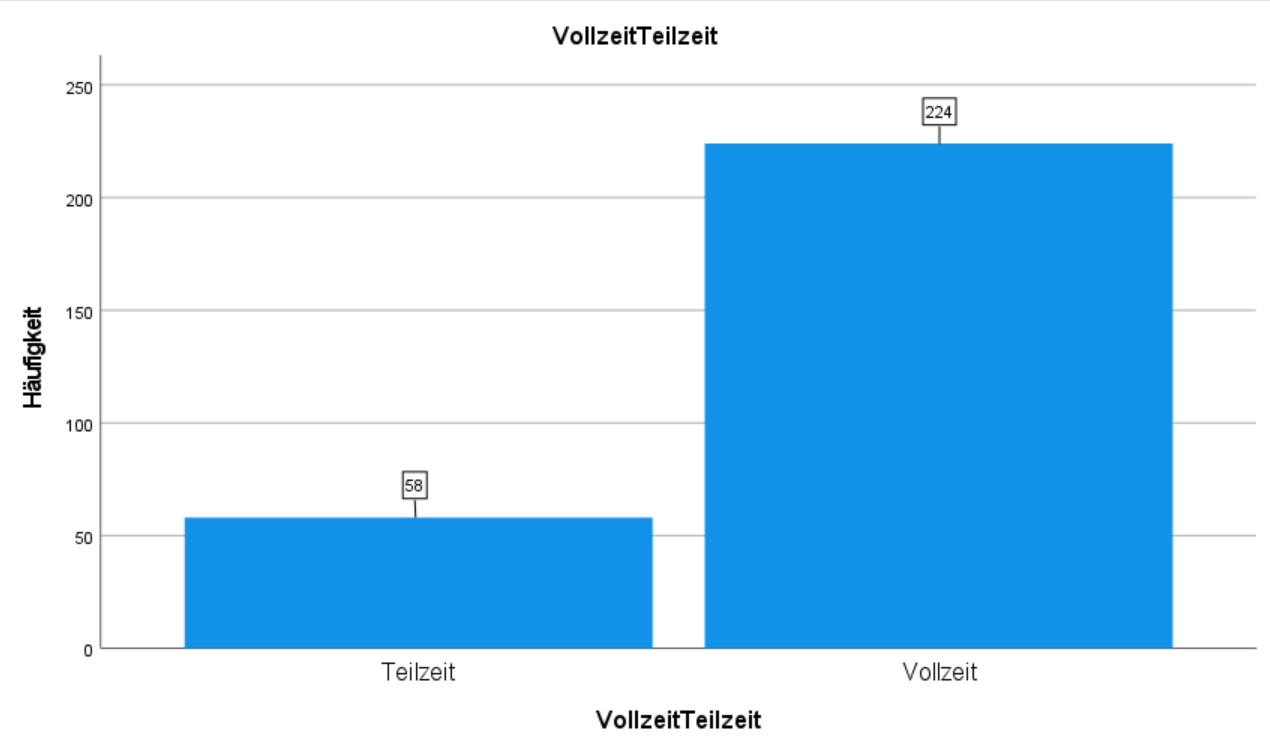
\includegraphics[width=\textwidth]{04_Artefakte/01_Abbildungen/deskriptiv_teilzeit_vollzeit.png}
        \caption{Berufssituation der Teilnehmenden}
        \label{fig:berufssituation}
    \end{subfigure}
    \begin{subfigure}{0.49\textwidth}
        \centering
        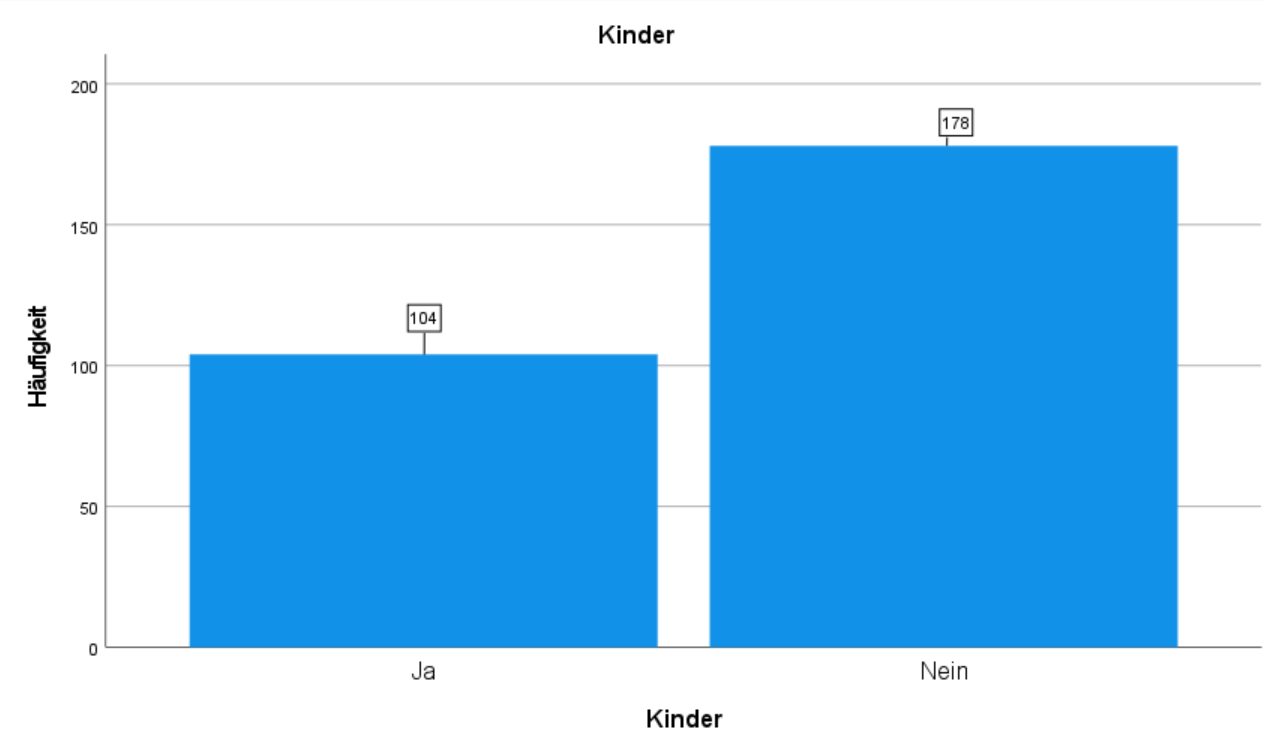
\includegraphics[width=\textwidth]{04_Artefakte/01_Abbildungen/deskriptiv_kinder.png}
        \caption{Anzahl der Teilnehmenden mit Kindern}
        \label{fig:kinder}        
    \end{subfigure}
\end{figure}

Als Teil der Umfrage haben außerdem 104 Personen angegeben, dass sie Kinder haben. Dies entspricht einem Anteil von 36,9\% der 
Teilnehmenden (siehe Abbildung \ref{fig:kinder}).

Bezogen auf die berufliche Situation der Befragten, haben 79,4\% der Teilnehmenden angegeben, dass sie in 
Vollzeit arbeiten. 20,6\% der Teilnehmenden arbeiten in Teilzeit (vgl. Abbildung \ref{fig:berufssituation}).

\begin{figure}[h]
    \centering
    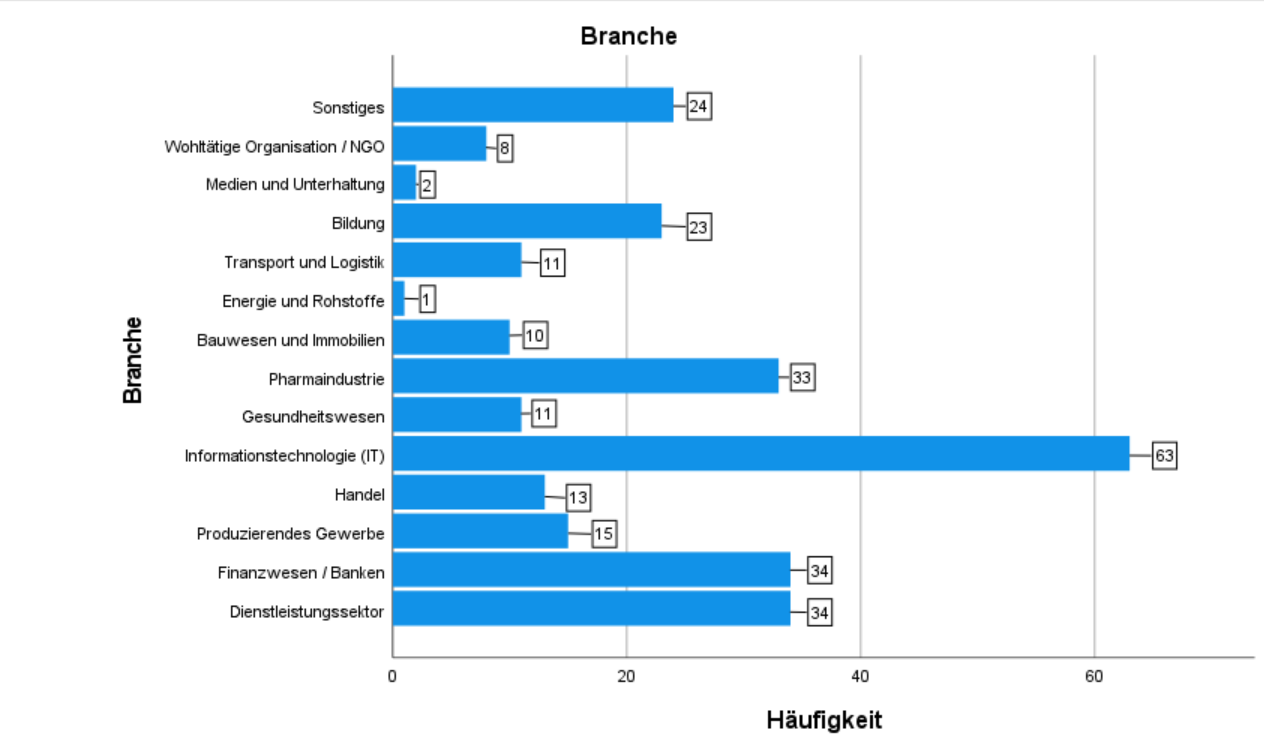
\includegraphics[width=0.9\textwidth]{04_Artefakte/01_Abbildungen/deskriptiv_branche.png}
    \caption{Branchenverteilung der Teilnehmenden}
    \label{fig:branche} 
\end{figure}

\begin{figure}[h]
    \centering
    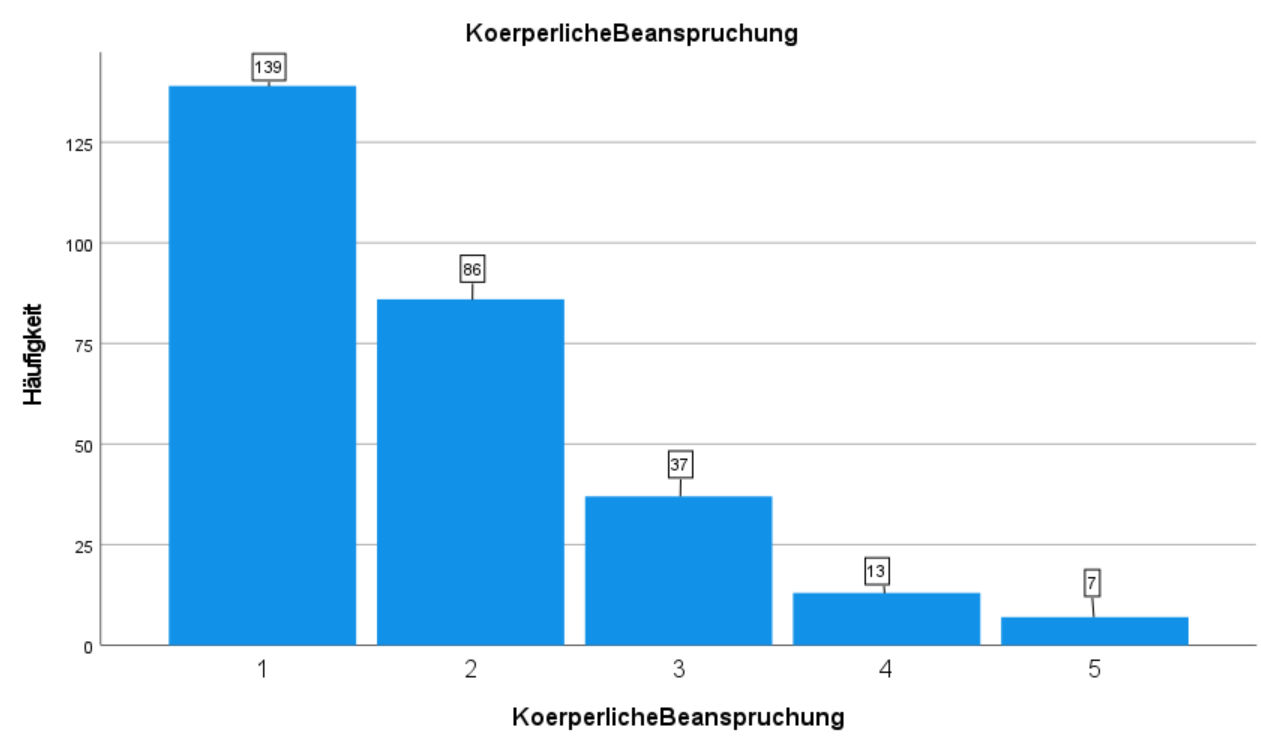
\includegraphics[width=0.5\textwidth]{04_Artefakte/01_Abbildungen/deskriptiv_koerperliche_beanspruchung.png}
    \caption{Körperliche Beanspruchung der Arbeit der Teilnehmenden}
    \label{fig:koerperliche_beanspruchung}
\end{figure}
Des Weiteren ist zu beobachten, dass eine starke Mehrheit der Befragten aus der IT Branche (vgl. Abbildung \ref{fig:branche}) 
kommen und ihre Arbeit als wenig körperlich anstrengend empfinden (vgl. Abbildung \ref{fig:koerperliche_beanspruchung}).

